\documentclass[12pt]{report}
\usepackage[top=3.0cm, bottom=3.0cm, left=3.0cm, right=3.0cm]{geometry}
\usepackage{enumerate}
\usepackage{graphicx}
\usepackage{algorithmic}
\usepackage[ruled,vlined]{algorithm2e}
\usepackage{multirow}
\usepackage{amsmath}
\usepackage{setspace}
\usepackage{subfig}
\usepackage{url}
\usepackage{parskip}
\usepackage{fancyhdr}
\usepackage{fancyvrb}
\usepackage{hyperref}
\usepackage{listings}
\usepackage[svgnames]{xcolor}
\usepackage{lineno}
\usepackage{soul}
\usepackage{array}
\usepackage{environ}
\usepackage{booktabs}
\usepackage{longtable}
\usepackage{float}
\usepackage{makeidx}
\makeindex

\setlength\parindent{0pt}
\setlength{\headheight}{15pt}
\emergencystretch=2em
\newcommand{\etal}{\textit{et al. }}
\NewEnviron{myequation}{\begin{equation}\scalebox{1.4}{$\BODY$}\end{equation}}

\definecolor{codegreen}{rgb}{0,0.45,0}
\definecolor{codegray}{rgb}{0.42,0.42,0.42}
\definecolor{codepurple}{rgb}{0.48,0,0.68}
\definecolor{backcolour}{rgb}{0.95,0.95,0.92}
\lstdefinestyle{mystyle}{
    backgroundcolor=\color{backcolour},
    commentstyle=\color{codegreen},
    keywordstyle=\color{blue},
    numberstyle=\tiny\color{codegray},
    stringstyle=\color{codepurple},
    basicstyle=\ttfamily\small,
    breaklines=true,
    captionpos=b,
    keepspaces=true,
    numbers=left,
    numbersep=5pt,
    showspaces=false,
    showstringspaces=false,
    showtabs=false,
    tabsize=4
}
\lstset{style=mystyle}

\newenvironment{certificate}{\centering}{}
\newenvironment{abst}{\centering\doublespacing}{}
\newenvironment{dedication}{
\clearpage\centering\thispagestyle{empty}\vspace*{\stretch{1}}\raggedleft\setstretch{2.0}
}{\par\vspace{\stretch{4}}\clearpage}

\begin{document}

\thispagestyle{empty}
\begin{center}
    \begin{minipage}{1.1\linewidth}
        \centering
        {{\Large \textbf{AI-Based Phishing Detection System\\Using Ensemble Learning}}}\\
        \vspace{1.0cm}
        {\textit{A report submitted in partial fulfillment of the requirements \\ for the award of the degree of}\\
        \vspace{1.5cm}
        \bfseries Bachelor of Technology\\
        in\\
        Computer Science \& Information Technology}
        \vspace{1.0cm}
        \begin{center}
            \large \textbf{by}
        \end{center}
        \vspace{0.5cm}
        \begin{center}
        \begin{tabular}{l l}
        \textbf{D Sunidhi} & \textbf{2320090017} \\[8pt]
        \textbf{P Manvitha} & \textbf{2320090060} \\[8pt]
        \textbf{G Likith} & \textbf{2320090069} \\[8pt]
        \end{tabular}
        \end{center}
        \vspace{1.0cm}
        {\large Under the Supervision of \par \textbf{Dr. K Venkateshwara Rao}\\}
        \vspace{1.0cm}
        {\centering
\includegraphics[scale=0.7]{images/logo.png}}

        \normalsize \textbf{KONERU LAKSHMAIAH EDUCATION FOUNDATION, BOWRAMPET\\
        \vspace{0.5cm}
        Hyderabad-500043, Telangana, India}\\
        \vspace{0.5cm}
        \normalsize Academic Year 2026--2027
    \end{minipage}
\end{center}
\clearpage

\begin{certificate}
    \clearpage
    {\centering
\includegraphics[scale=0.93]{images/header.png}}
    \thispagestyle{empty}
    \underline{\textbf{CERTIFICATE}}
\end{certificate}
\par\null\par
\begin{doublespace}
This is to certify that \textbf{D Sunidhi} (ID No. \textbf{2320090017}),
\textbf{P Manvitha} (ID No. \textbf{2320090060}), and
\textbf{G Likith} (ID No. \textbf{2320090069}), B.Tech students of
Computer Science \& Information Technology, have worked on the project
entitled \textbf{``AI-Based Phishing Detection System Using Ensemble Learning''}
under my supervision and guidance. The content of this report is original
and has not been submitted elsewhere for the award of any academic or
professional degree.
\end{doublespace}

\par\null\par\par\null\par\par\null\par\par\null\par
\begin{flushleft}
.........................................................\\
\par\null\par
\textbf{Dr. K Venkateshwara Rao}\\
Project Guide,\\
Department of Computer Science \& Information Technology,\\
Koneru Lakshmaiah Education Foundation, Telangana, India\\
Bowrampet, Hyderabad-500043\\
\end{flushleft}
\par\null\par\par\null\par
Date: ........................


\pagenumbering{roman}
\newpage
\begin{abst}
    \thispagestyle{empty}
    \section*{Acknowledgments}
\end{abst}
\doublespacing
We express our sincere gratitude to our project guide, Dr. K Venkateshwara
Rao, for his direction, critical feedback, and encouragement throughout this
work. His guidance helped us move from a simple reproduction exercise to a
carefully audited system with explicit data provenance, domain-separated
evaluation, robustness testing, and a deployable demonstration.

We thank the faculty and staff of the Department of Computer Science \&
Information Technology, Koneru Lakshmaiah Education Foundation, Bowrampet,
for providing the academic environment and facilities required to complete
the project. We also acknowledge the authors of the reference PhishX study,
the maintainers of PhishTank and Tranco, and the developers of the open-source
software used in the implementation, including Python, PyTorch, LightGBM,
FastAPI, scikit-learn, ONNX Runtime, and the supporting scientific libraries.

Finally, we thank our families and classmates for their continued support.
Every claim and metric in this report has been checked against the preserved
source code or saved experimental artifacts. Any remaining limitations are
stated openly so that this report can serve as a reproducible academic record
rather than only a demonstration of a high headline accuracy.

\thispagestyle{empty}
\addcontentsline{toc}{chapter}{Acknowledgments}

\newpage
\begin{abst}
    \thispagestyle{empty}
    \section*{Abstract}
\end{abst}
\doublespacing
This report presents a versioned study of an AI-based phishing detector. The first experiment independently reproduced a character-level CNN and 36-feature LightGBM ensemble on 20,000 URLs. The deployed application later adopted a character CNN, two-layer bidirectional LSTM and additive attention. A source-level audit found that the newer trainer did not preserve the original root-domain separation guarantee. Whole-domain reservations, consistent cleaned-input identity and frozen split hashes were therefore introduced before a separately versioned v3.4 training run.

The corrected experiment retains 63,869 records: 25,961 training, 6,113 validation and 31,795 test records. All pairwise hostname and registered-domain intersections are zero. At threshold 0.5, the candidate achieves 92.876\% test accuracy, 90.696\% recall and 98.289\% ROC-AUC, with 718 false positives and 1547 false negatives. The frozen validation gate failed. The current deployed model remains v3.3; candidate research results are not presented as deployed performance.

Independent HTML and email analyzers provide contextual warning signals without visiting destinations, executing pasted HTML or accessing a mailbox. Human-verified feedback, model versioning, deterministic robustness tests and drift-monitoring infrastructure extend the initial URL-only reproduction. Their scope and limitations are documented separately from classifier accuracy. The report emphasizes reproducible evidence and honest trade-offs rather than assuming that more data or a newer architecture necessarily improves every metric.
\thispagestyle{empty}
\addcontentsline{toc}{chapter}{Abstract}

\newpage
\tableofcontents
\addcontentsline{toc}{chapter}{\listtablename}
\listoftables
\cleardoublepage
\addcontentsline{toc}{chapter}{\listfigurename}
\listoffigures
\cleardoublepage

\clearpage
\pagenumbering{arabic}
\doublespacing
\pagestyle{fancy}
\fancyhf{}
\fancyhf[loh,reh]{\slshape\rightmark}
\fancyhf[leh,roh]{\thepage}
\renewcommand*\headrulewidth{1pt}

\hypersetup{urlcolor=blue,linkcolor=blue,citecolor=red}

\chapter{Introduction}
\section{Project Context and Problem Statement}
Phishing uses deceptive messages and destinations to persuade users to disclose information or take unsafe actions. A URL-only classifier can screen a link before any webpage is downloaded. Its limitation is equally important: a string does not reveal all aspects of the destination, ownership, content or intent. A familiar domain name in a URL can appear in a misleading path, while a legitimate account page can contain suspicious-looking terms.

False alarms on ordinary URLs and earlier root-slash instability motivated production changes. Those changes also made historical reports incomplete descriptions of the live API.

\section{Objectives}
The objectives are to reproduce the reference URL ensemble independently; identify the exact current neural architecture; prevent data leakage through complete registered-domain grouping; compare accuracy, precision, recall, F1, ROC-AUC and error counts; evaluate deterministic synthetic mutations; and explain safe HTML/email evidence independently of the URL probability. A further objective is to prevent unverified feedback from automatically becoming training truth.

\section{Version History and Scope}
The original reference is PhishX \cite{dubey2025phishx}. Our first reproduction used 20,000 URLs and a validation-selected 95/5 CNN--LightGBM mixture. A historical robustness candidate reduced synthetic phishing misses from 37 to 17 on its own test. Production V2 later used new models at 35/65. Current production v3.3 instead uses CNN--BiLSTM--attention for the verdict. The v3.4 repair keeps that network but changes data partition integrity.

These stages are not interchangeable. The title of the college project retains the original ensemble-learning identity, but current implementation chapters explicitly distinguish the reference ensemble from the neural production verdict. This report is dated October 13, 2026, and does not overwrite the historical report PDF.


\chapter{Literature Survey and Existing System}
\section{Literature Survey}
Table \ref{tab:lit} summarizes nineteen relevant studies. The comparison describes their methods, not an artificial cross-dataset accuracy ranking. The current project does not claim to invent convolution, recurrence, attention or human review.
\begin{singlespace}\small
\begin{longtable}{p{0.24\textwidth}p{0.32\textwidth}p{0.34\textwidth}}
\caption{Relevant literature and its relationship to this project}\label{tab:lit}\\
\toprule Study & Focus & Project relationship\\\midrule\endfirsthead
\toprule Study & Focus & Project relationship\\\midrule\endhead
Dubey et al. \cite{dubey2025phishx} & Character CNN plus 36-feature LightGBM & Direct reference for the first independent reproduction; not the current recurrent verdict.\\
Khonji et al. \cite{khonji2013survey} & Survey of phishing detection & Frames the diversity of URL, content and user-facing approaches.\\
Ma et al. \cite{ma2009blacklists} & Learning suspicious URL patterns beyond lists & Motivates generalization beyond exact known destinations.\\
Garera et al. \cite{garera2007framework} & Detection and measurement of phishing & Establishes URL-related evidence as an earlier research direction.\\
Blum et al. \cite{blum2010lexical} & Lexical URL features and online learning & Adaptation is prior work; our reviewed workflow is a prototype, not a new learning theory.\\
Zhang et al. \cite{zhang2007cantina} & Content-based phishing detection & Content can supplement URL evidence, but our text parser does not reproduce its detector.\\
Xiang et al. \cite{xiang2011cantina} & Feature-rich content learning & Demonstrates richer evidence; our standalone HTML signals are uncalibrated.\\
Sahoo et al. \cite{sahoo2017survey} & Malicious URL detection survey & Provides a taxonomy of representation and data challenges.\\
Saxe and Berlin \cite{saxe2017expose} & Character embeddings and convolution & Related character-pattern learning without manual tokenization.\\
Le et al. \cite{le2018urlnet} & Learned character and word URL representations & Our model has no URLNet word branch; representation choices differ.\\
Bahnsen et al. \cite{bahnsen2017rnn} & Recurrent phishing URL classification & Sequence modeling for URLs predates our BiLSTM extension.\\
Sahingoz et al. \cite{sahingoz2019machine} & Machine learning from URLs & Shows the role of extracted URL representations and comparative evaluation.\\
Jain and Gupta \cite{jain2018client} & Client-side machine-learning detection & Related deployment setting; this project uses a server API.\\
Mohammad et al. \cite{mohammad2014predicting} & Self-structuring neural detection & Neural phishing classification is established prior work.\\
Fette et al. \cite{fette2007email} & Learning phishing email detection & Our email tool is not a trained equivalent and has no measured email accuracy.\\
Zhang et al. \cite{zhang2015character} & Character CNN text classification & Motivates local character-feature extraction.\\
Ke et al. \cite{ke2017lightgbm} & Efficient gradient-boosted trees & Supplies the established engineered-feature model.\\
Hochreiter and Schmidhuber \cite{lstm} & Gated long short-term memory & Basis for the implemented recurrent component.\\
Schuster and Paliwal \cite{brnn} & Bidirectional recurrent networks & Basis for using both sequence directions.\\\bottomrule
\end{longtable}\end{singlespace}

\section{Existing System and Gap}
The reference article reports a 60/40 CNN--LightGBM ensemble, approximately 99,361 URLs, and 99.819\% accuracy on its test. It describes 70 symbols and embedding width 128. The released implementation and our original reproduction differ in some metadata; our historical encoder has 49 explicit characters and embedding width 16. This report uses source code for our implementation, rather than copying the reference architecture values into our tables.

The reference identifies adversarial robustness and richer content/context as future directions. Our extensions address bounded versions of those directions. Deterministic strings provide reproducible stress tests, while pasted HTML/email provides supplementary evidence without unsafe fetching. The newest revision adds recurrence and attention but does not establish that either is a novel algorithm.

\section{Evaluation and Calibration Lessons}
Tranco is designed as a research-oriented ranking \cite{lepochat2019tranco}; a popular root is still not equivalent to every legitimate path. Neural confidence also need not be calibrated \cite{guo2017calibration}. Adding a sigmoid supplies a probability-shaped score, not proof of calibration. Learned attention weights \cite{attention} are aggregation parameters, not a causal explanation of why a website is malicious. These distinctions guide the implementation and the claims made in later chapters.

\chapter{Data Collection and Preprocessing}
\section{Source Data and Labels}
The original 20,000-URL reproduction sampled balanced classes from frozen PhishTank- and Tranco-derived snapshots \cite{phishtank,lepochat2019tranco}. Later production work used a 40,000-row balanced dataset. The v3.3 source pool added 24,000 records: 12,000 phishing URLs, 9,000 legitimate paths and 3,000 lower-ranked legitimate roots. The source labels are inherited; no destination was fetched to independently relabel it.

The existing cleaner repairs selected scraping artifacts, including escaped percent symbols and HTML ampersands, removes enclosing quote artifacts and rejects invalid hosts or internal whitespace. The repaired partitioner shares cleaning-based exclusion semantics with future snapshot construction. It retains 63,869 records after 81 invalid rows and 50 duplicate rows are excluded. Source CSVs and prior experiment results remain unchanged.

A conservative identity key lowercases and ignores a leading scheme and www prefix for deduplication. This is an exclusion safeguard, not the model input. The actual neural encoder preserves path/query case after production canonicalization.

\section{Canonicalization and Encoding}
The production boundary trims whitespace, adds HTTPS when a scheme is missing, normalizes scheme and host case, removes default ports, and equates an empty root path with a slash-only root path. A non-root trailing slash is preserved. Query parameters, fragments and percent encodings are not broadly rewritten. RFC 3986 provides the URI context \cite{rfc3986}. Processing is string-only.

The first CNN retained the rightmost 200 lowercased characters from its 49-symbol explicit alphabet, with PAD 0 and UNK 50. The current recurrent family uses 95 printable ASCII symbols, PAD 0 and UNK 96, first-256 truncation and right padding. The v3.4 repair does not alter that current model representation.

\section{Leakage Discovery and Whole-Domain Repair}
The previous trainer assigned individual hard-negative or previous-test URLs before grouping other records. This allowed a domain already reserved for test to have another URL placed in training. v3.3 reconstructed overlaps were 11/40/6 by hostname and 385/400/187 by private-suffix registered domain. Exact URL-key intersections alone were zero and therefore failed to expose the issue. Two external snapshot inputs also matched cleaned training strings.

The corrected policy uses public-suffix registered domains, deliberately grouping private-hosting tenants together. IP hosts are handled explicitly. Domain reservations are resolved as test greater than validation greater than training. All members inherit the chosen split. Domains from previous test and external snapshots are excluded from candidate training; remaining groups are assigned with seed-42 stratified group folds. Assertions cover hostname, public domain, private domain and key intersections.

\begin{table}[H]\centering\caption{Actual corrected v3.4 partitions}
\begin{tabular}{lrrr}\toprule Partition & Legitimate & Phishing & Total\\\midrule
Train & 13,612 & 12,349 & 25,961\\Validation & 3,220 & 2,893 & 6,113\\Test & 15,168 & 16,627 & 31,795\\\bottomrule\end{tabular}\end{table}
All pairwise domain overlaps are zero. Previously evaluated domains take priority over a desired ratio. Assignment hashes were frozen before training; the snapshots remain previously inspected evidence.

\section{Engineered Features}
The historical/reference LightGBM branch still uses 36 values: length and character-composition measures, structural punctuation and segments, hostname/path entropy, suspicious TLDs, six length buckets, and nine keyword indicators (login, signin, secure, webscr, bank, verify, update, account and confirm). No DNS lookup, WHOIS data, rendered logo or page content is part of this vector. These features remain useful for describing a URL but do not explain the current BiLSTM verdict causally.


\chapter{Proposed Approach, Implementation and Results}
\section{Current System Architecture}
Figure \ref{fig:system} separates production v3.3 from legacy reference scores and independent context evidence. The unpromoted v3.4 candidate uses the same network.
\begin{figure}[htbp]\centering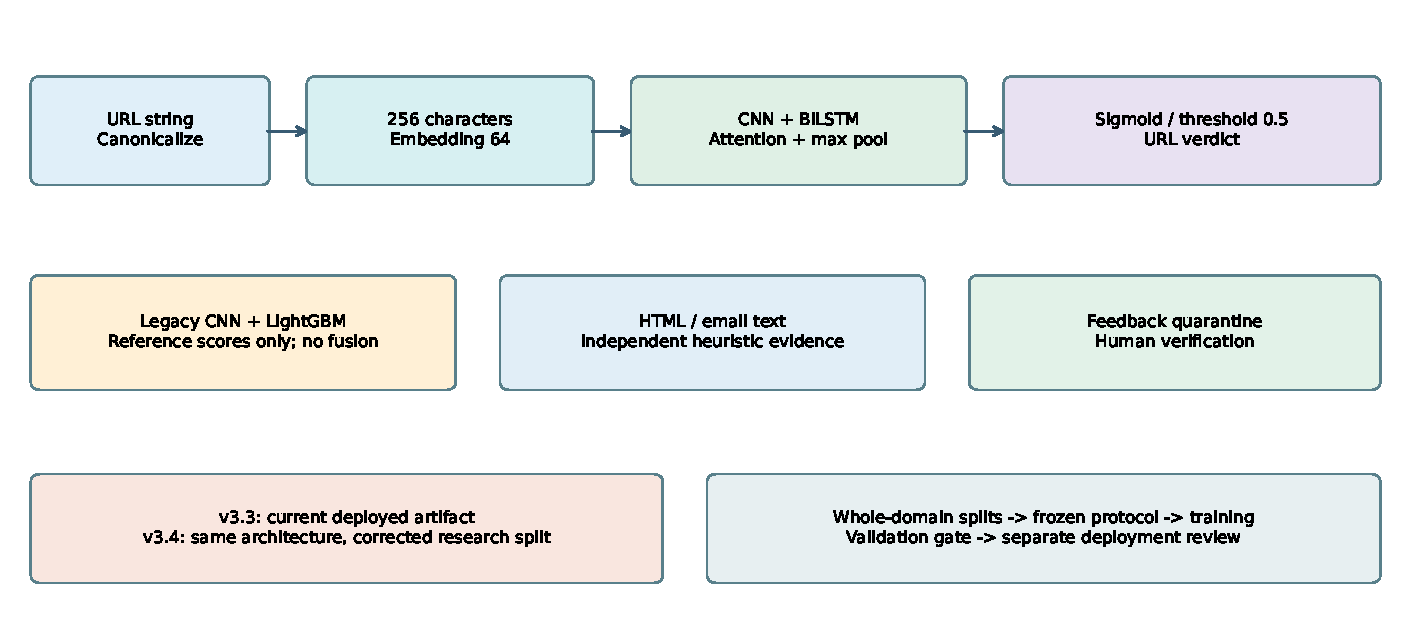
\includegraphics[width=.90\textwidth]{images/system_architecture.pdf}\caption{Versioned classifier and independent extensions}\label{fig:system}\end{figure}

\section{CNN--BiLSTM--Attention Network}
Character indices enter a 64-dimensional embedding. Parallel kernels 3, 5 and 7 each have 128 convolutional channels, BatchNorm and ReLU. Their 384 concatenated channels are max-pooled by two, producing 128 time steps from 256 input positions. Dropout 0.2 precedes the recurrent component. The LSTM has two layers, input width 384, hidden width 128 per direction and a true bidirectional flag. Its output width is 256 at each time step.

Additive attention maps 256 values to 64 and then one score, applies tanh and a time-axis softmax, and computes a weighted sum. This 256-vector is concatenated with a temporal maximum to form 512 values. The classifier has widths 512, 128, 32 and 1, LayerNorm, ReLU, dropout 0.3/0.15 and final sigmoid. There are 1,138,434 parameters. It is not multi-head transformer attention and does not mask padding explicitly.
\begin{figure}[htbp]\centering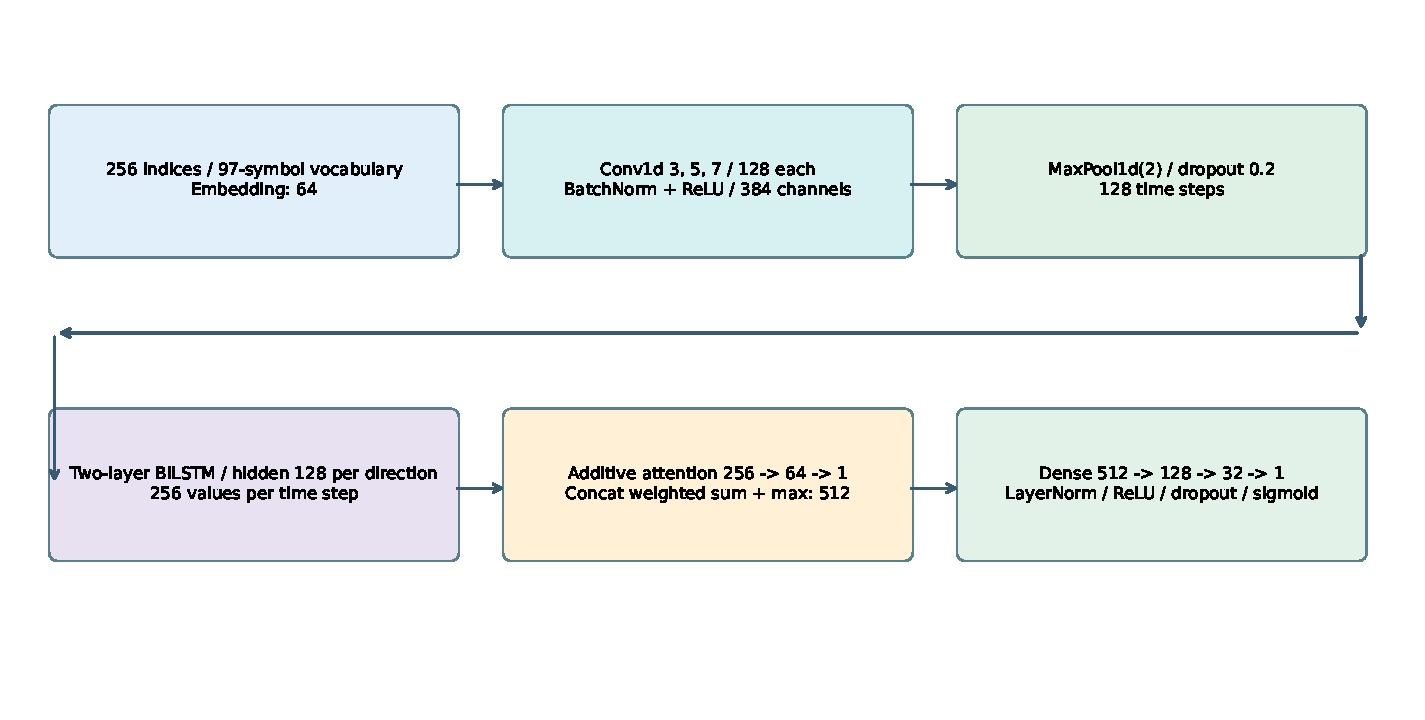
\includegraphics[width=\textwidth]{images/new_model_architecture.pdf}\caption{Exact implemented recurrent architecture}\end{figure}

The original CNN summarized local character patterns with global pooling. The new network retains a sequence of CNN features and reads it in both directions before aggregation. This can model relationships among hostname, path and other character patterns. The theoretical capability does not establish a measured improvement from bidirectionality alone: data, encoding and training exposure also changed between project versions.

\section{Ensemble History}
The reference mixture weights CNN and LightGBM at 60/40. The first independent experiment selected 95/5 on validation AUC. Production V2 later used separately trained artifacts at 35/65. In current production, these component outputs are returned as reference values, while the recurrent probability determines the verdict. The current neural model is therefore not described as a newly calibrated CNN--LightGBM ensemble.

\section{Safe Context and Reviewed Adaptation}
HTML parsing detects structural evidence such as forms, passwords, script/iframe tags, redirect metadata and credential terms. Standalone HTML has no base URL; an absolute target is not proof of cross-origin theft. Email analysis recognizes implemented risk phrases, credential requests, calls to action and URL strings. Neither tool executes code or accesses a mailbox. Both return qualitative evidence rather than validated ML confidence.

Feedback enters quarantine and requires human verification. An approved dataset can feed an explicitly invoked candidate-training process, followed by validation and model versioning. PSI monitors engineered-feature distributions; it does not itself prove an attack or model failure. The project has infrastructure for controlled adaptation, not demonstrated autonomous online learning.
\section{Training Configuration and Freeze}
The repaired experiment was frozen in commit \texttt{5543066} before model fitting. Dataset, split and implementation hashes guard against silent changes. Seed 42, CPU/four threads, batch size 128, AdamW with learning rate 0.001 and weight decay 0.0001, BCEWithLogitsLoss and gradient clipping 5.0 are used. Training allows at most seven epochs with patience three on validation ROC-AUC. The scheduler halves the learning rate after one plateau. Epoch 7 was selected. The threshold stays 0.5.

\begin{lstlisting}[language=Python,caption={Whole-group reservation policy (simplified)}]
priority = {"train": 0, "validation": 1, "test": 2}
for url, requested_split in reservations:
    group = registered_domain(clean(url))
    fixed[group] = higher_priority(fixed.get(group), requested_split)
for row in rows:
    row.split = fixed.get(row.group, grouped_fold[row.group])
assert train_domains.isdisjoint(validation_domains)
assert train_domains.isdisjoint(test_domains)
assert validation_domains.isdisjoint(test_domains)
\end{lstlisting}
This simplified policy illustrates the local research experiment; it is not production code.

\section{Serving, Interface and Testing}
The selected PyTorch checkpoint is exported to ONNX with dynamic batch size and checked against PyTorch outputs. The model config records an SHA-256 digest. Production rejects missing or mismatched artifacts rather than falling back silently. Training needs PyTorch; the web runtime uses ONNX Runtime and does not require training libraries. The candidate is saved under new v3.4 filenames, leaving v3.3 unchanged.

The FastAPI application exposes health, model information, URL prediction, combined context, independent HTML/email analysis and feedback. Each tool has a separate input/action/result. The browser never needs to open a submitted suspicious destination. Public deployment remains at the existing Vercel project. The source repository and deployment URL identify the demonstration, while saved checkpoint/version records identify the experiment.

The current production-source suite passes 91 tests. The separate local research branch previously passed 107, including reservation and frozen-split assertions. These checks establish software behavior, not universal prediction accuracy. Candidate models and training changes remain local; only final documents and supporting evidence are published.

\section{Promotion Decision}
Candidate checkpoint selection uses validation only. The predeclared comparison gate requires no loss in validation AUC or recall against v3.3 and no more than a one-percentage-point benign false-positive-rate increase. The gate failed. No model is automatically promoted by this branch. The old deployment's explicit maintainer override is documented rather than presented as a passed gate. Previously inspected test outcomes do not trigger another threshold or epoch search.
\section{Corrected Candidate Results}
The domain-separated candidate has 92.876\% accuracy, 95.455\% precision, 90.696\% recall, 93.015\% F1, 98.289\% ROC-AUC and 98.419\% average precision on 31,795 test rows. There are 718 false positives and 1547 false negatives at threshold 0.5. Zero domain overlap is an integrity property, not a promise of near-perfect accuracy.
\begin{figure}[htbp]\centering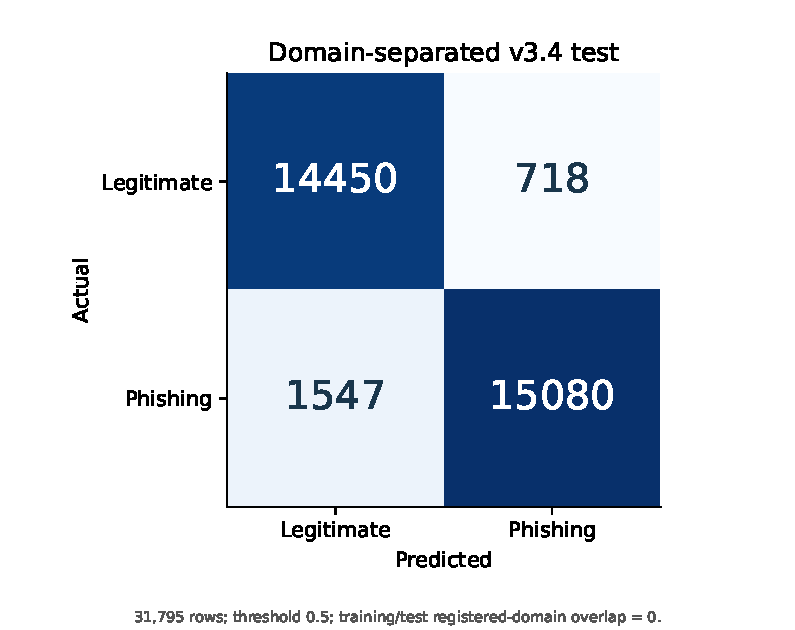
\includegraphics[width=.66\textwidth]{images/confusion_matrix.pdf}\caption{Candidate test confusion matrix}\end{figure}

\section{Common External Snapshot}
The existing fresh2 snapshot has 11,273 rows; two exceed the API's 2,048-character limit. All comparison rates use the remaining 11,271 strings. Before repair, V2 produced 2,177 false positives and 467 false negatives; v3.3 produced 384 and 547. The candidate's external accuracy is 90.578\% and recall 88.232\%. These observations describe different training histories, not a matched architecture ablation.
\begin{figure}[htbp]\centering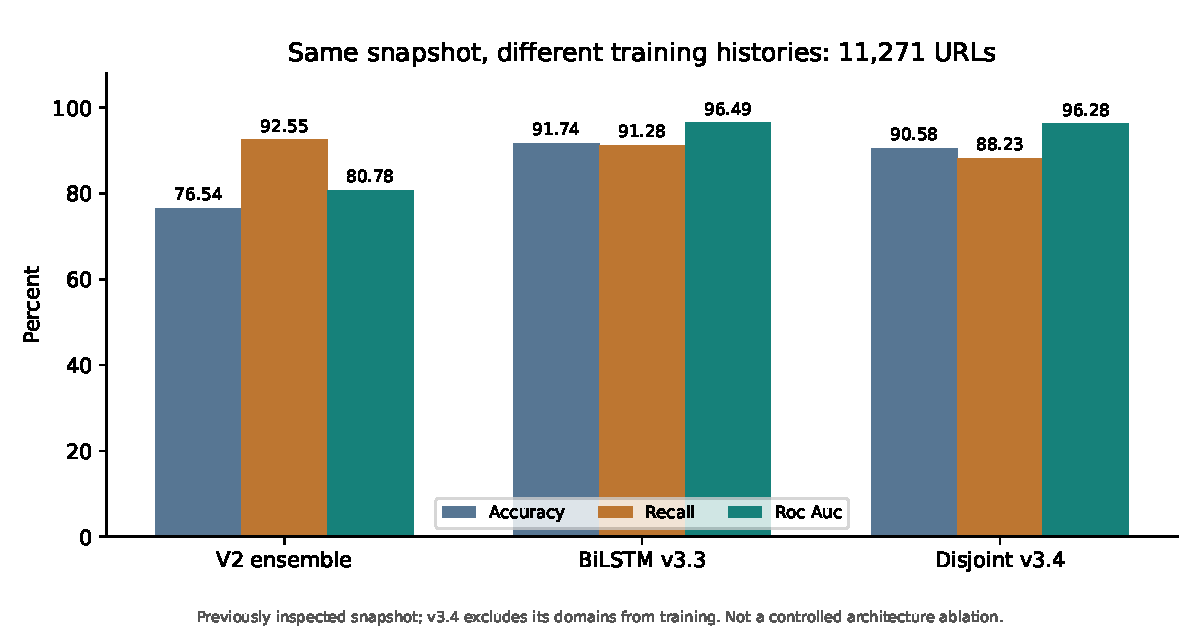
\includegraphics[width=\textwidth]{images/model_comparison.pdf}\caption{Common-input external comparison; snapshot previously inspected}\end{figure}

\section{Adversarial Stress Results}
The old synthetic set contains 1,995 mutated phishing strings and 2,003 unchanged benign strings. V2 misses 9 phishing URLs and v3.3 misses 119. The corrected candidate misses 173, with 91.328\% recall. It was not adversarially fine-tuned during this repair. The historical 37-to-17 result concerns another candidate and cannot be reused as the new model's result.
\begin{figure}[htbp]\centering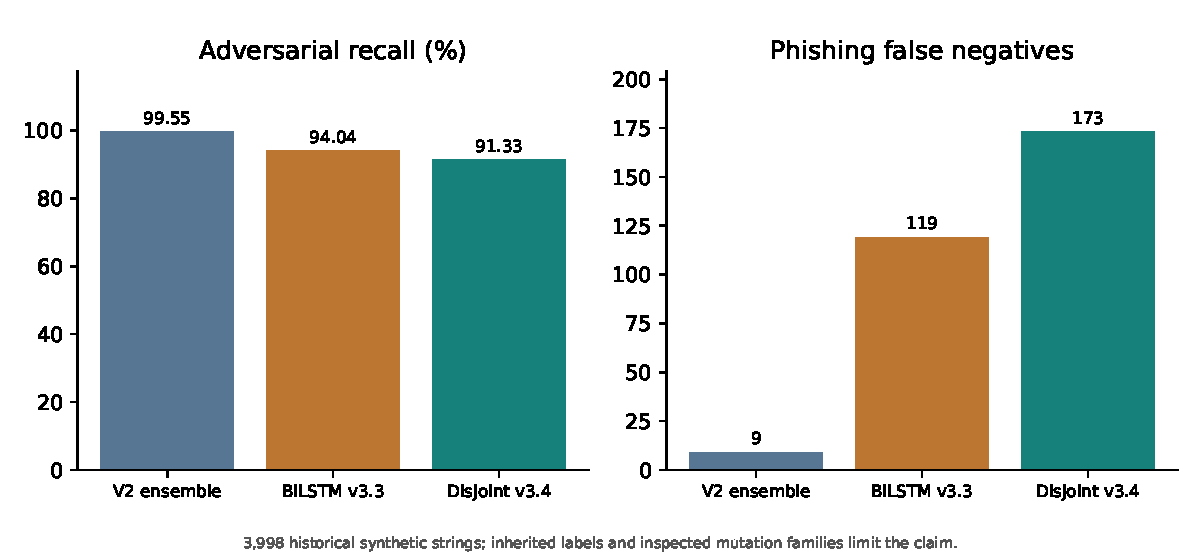
\includegraphics[width=\textwidth]{images/adversarial_robustness.pdf}\caption{Synthetic robustness comparison with explicit false-negative counts}\end{figure}

\section{Training Evidence}
Both losses and validation AUC are saved for the new run. Test scores do not choose an epoch. Figure \ref{fig:history} reflects the recorded history rather than an illustrative curve.
\begin{figure}[htbp]\centering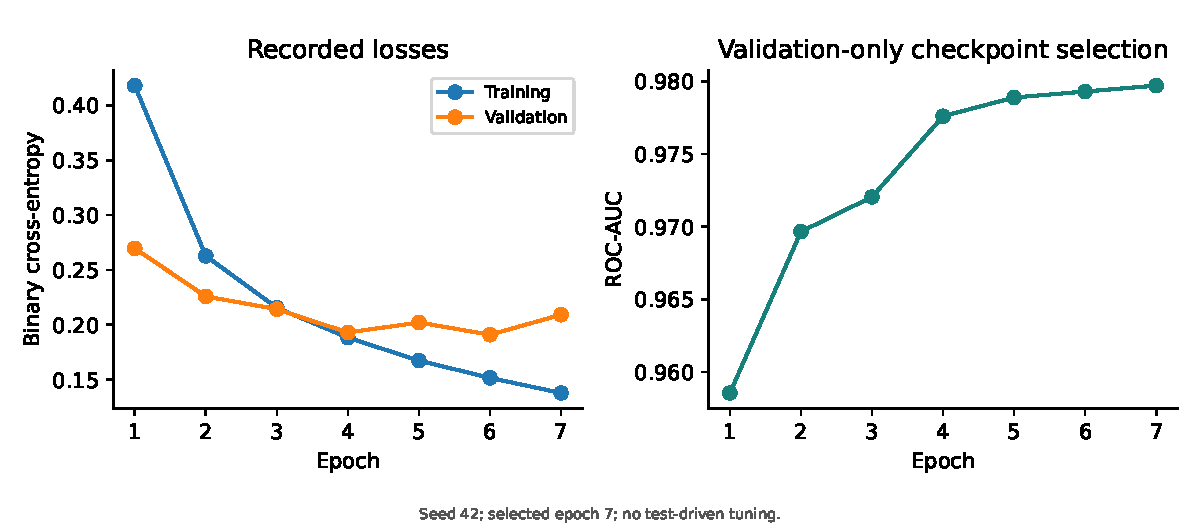
\includegraphics[width=\textwidth]{images/training_history.pdf}\caption{Actual v3.4 training history}\label{fig:history}\end{figure}

\section{Reference Study and Historical Reproduction}
The paper reports 99.819\% accuracy, 100\% precision, 99.635\% recall and 99.947\% ROC-AUC. Our first 20,000-URL reproduction reports 99.525\%, 100\%, 99.048\% and 99.931\% respectively on its 3,998-row test. The candidate values above use a different corpus and partition. These numbers are separately labelled and are not used to claim that one study dominates another. Complete current comparisons, including PR-AUC, FP and FN, are stored in \texttt{docs/evidence/latest\_model\_comparison.csv}.
\section{What Improved and What Did Not}
The repair improves evaluation integrity: group reservations can no longer leak an already reserved domain into another split, and future snapshot exclusions use cleaning-aware identities. It does not guarantee increased accuracy. The current production revision reduces many external false alarms relative to V2 but sacrifices some recall and performs worse on the historical mutation set. The corrected candidate must be judged on its own saved rows and declared validation rule, not on a preferred conclusion.

\section{Known Limitations}
The dataset inherits source labels and may contain source-specific cues. No newly collected temporal holdout, multiple-seed study or matched-training architecture ablation was conducted. Domain separation does not remove shared campaigns across different domains. Public-suffix grouping can reserve an entire hosting provider, and many previously evaluated groups make the candidate test partition unusually large. These are disclosed design choices.

The external snapshots were inspected before repair and are not prospectively unseen. Earlier models may have trained on domains in the corrected candidate test, so their same-input scores are diagnostic. Small ranking-metric discrepancies between old saved and batched-replay scores are retained rather than hidden. Classification counts reproduce; the cause of every numerical difference is not established.

The neural output is not separately calibrated. First-256 truncation can hide late URL information, and unmasked padding may influence recurrence. Attention weights are not verified explanations. Synthetic mutations inherit labels without a live functionality check. HTML/email signals are unvalidated heuristics; feedback review and PSI infrastructure have not been demonstrated as long-term autonomous learning or poisoning resistance.


\chapter{Conclusion and Future Scope of Work}
\section{Conclusion}
Production uses CNN--BiLSTM--attention v3.3, whose audit exposed domain leakage and cleaned-input contamination. The earlier v3.4 research run repaired domain separation: test accuracy was 92.876\% and recall 90.696\%. It failed promotion. Production remains v3.3; this output refresh performs no training or deployment.

\section{Future Scope}
Priorities are new temporal data, matched baselines, multiple seeds, component ablations and calibration. HTML/email fusion needs labelled content; feedback needs longitudinal and poisoning studies. More similar URLs alone cannot guarantee generalization.


\onehalfspacing
\addcontentsline{toc}{chapter}{Bibliography}
\bibliographystyle{IEEEtran}
\bibliography{references}

\end{document}
